%&<latex>
\documentclass[letterpaper,12pt]{article}

%%%%%%%%%%%%%%%%%%%%%%%%%%%%%%%%%%%%%%%%%%%%%%%%%%%%%%%%%%%%
%% preamble %%%%%%%%%%%%%%%%%%%%%%%%%%%%%%%%%%%%%%%%%%%%%%%%
\pdfpagewidth = 8.5in
\pdfpageheight = 11.0in
\usepackage[left=1in,right=1in,top=1in,bottom=1in]{geometry}

\pagestyle{plain}
\pagenumbering{arabic}
\usepackage{setspace}
\usepackage[usenames]{color}
\usepackage[fleqn]{amsmath}
\usepackage{amssymb}
\usepackage{graphicx}
\usepackage{url}
\usepackage{verbatim}
\usepackage{appendix}
\usepackage{indentfirst}
\usepackage{booktabs}
\usepackage{multirow}
\usepackage[table, x11names]{xcolor}
\usepackage{ragged2e}
\usepackage{upgreek}
\usepackage{lscape}
\usepackage{longtable}
\usepackage[flushleft, referable]{threeparttablex}
\usepackage{rotating}
\usepackage[T1]{fontenc}
\usepackage[titles]{tocloft}
\usepackage{xspace}
\usepackage{ifthen}
\usepackage{cancel}
\usepackage{rotating}
\usepackage{array}
\usepackage{tabulary}
\usepackage{authblk}

\usepackage{hyperref}
\hypersetup{pdfborder={0 0 0}, colorlinks=true, urlcolor=black, linkcolor=black, citecolor=black}
\usepackage[capitalize]{cleveref}
\newcommand{\crefrangeconjunction}{--}

\usepackage[right, mathlines]{lineno}
\setlength\linenumbersep{1cm}
\def\linenumberfont{\normalfont\scriptsize\sffamily}

% \usepackage[format=plain, labelsep=period, justification=raggedright, singlelinecheck=true, skip=2pt, font=sf]{caption}
\usepackage{caption}
\DeclareCaptionLabelFormat{noSpace}{{#1}{#2}}
\DeclareCaptionListFormat{figList}{Figure {#2}.}
\DeclareCaptionListFormat{sFigList}{Figure S{#2}.}
\usepackage{subfig}

%\DeclareMathSizes{12}{12}{7}{5}

% \usepackage[round]{natbib}

% \makeatletter
%   \renewcommand{\section}{\@startsection{section}{1}{0mm}%
%     {-12pt}%
%     {12pt}%
%     {\sffamily\LARGE\itshape}}
% \makeatother

% \makeatletter
%   \renewcommand{\subsection}{\@startsection{subsection}{1}{0mm}%
%   {-10pt}%
%   {4pt}%
%   {\sffamily\large\bfseries\MakeUppercase}}
% \makeatother

% \makeatletter
%   \renewcommand{\subsubsection}{\@startsection{subsubsection}{1}{0mm}%
%   {-10pt}%
%   {10pt}%
%   {\sffamily\large\itshape}}
% \makeatother

% make list of figures ragged right
% \makeatletter
%   \renewcommand{\@tocrmarg}{0cm plus1fil}
% \makeatother

\setlength\linenumbersep{1cm}

% \newcommand{\change}[1]{{\color{blue} #1}\xspace}
\newcommand{\change}[1]{{\color{black} #1}\xspace}


\newcommand{\citationNeeded}{\textcolor{magenta}{\textbf{[CITATION NEEDED!]}}\xspace}
\newcommand{\tableNeeded}{\textcolor{magenta}{\textbf{[TABLE NEEDED!]}}\xspace}
\newcommand{\figureNeeded}{\textcolor{magenta}{\textbf{[FIGURE NEEDED!]}}\xspace}
\newcommand{\highLight}[1]{\textcolor{magenta}{\MakeUppercase{#1}}}

\newcommand{\editorialNote}[1]{\textcolor{red}{[\textit{#1}]}}
\newcommand{\ignore}[1]{}
\newcommand{\addTail}[1]{\textit{#1}.---}
\newcommand{\super}[1]{\ensuremath{^{\textrm{#1}}}}
\newcommand{\sub}[1]{\ensuremath{_{\textrm{#1}}}}
\newcommand{\dC}{\ensuremath{^\circ{\textrm{C}}}}

\providecommand{\e}[1]{\ensuremath{\times 10^{#1}}}

\newcommand{\mthnote}[2]{{\color{red} #2}\xspace}
\newcommand{\cwlnote}[2]{{\color{orange} #2}\xspace}

\newcommand{\ifTwoArgs}[3]{\ifthenelse{\equal{#1}{}\or\equal{#2}{}}{}{#3}\xspace}
\newcommand{\ifArg}[2]{\ifthenelse{\equal{#1}{}}{}{#2}\xspace}

%% New notation for divergence times
\newcommand{\divTime}[1]{\ensuremath{\tau_{#1}}\xspace}
\newcommand{\divTimeVector}{\ensuremath{\boldsymbol{\divTime{}}}\xspace}
\newcommand{\divTimeIndex}[1]{\ensuremath{t_{#1}}\xspace}
\newcommand{\divTimeIndexVector}{\ensuremath{\mathbf{\divTimeIndex{}}}\xspace}
\newcommand{\divTimeMap}[1]{\ensuremath{T_{#1}}\xspace}
\newcommand{\divTimeMapVector}{\ensuremath{\mathbf{\divTimeMap{}}}\xspace}
\newcommand{\divTimeScaled}[2]{\ensuremath{\mathcal{T}_{#1\protect\ifTwoArgs{#1}{#2}{,}#2}}\xspace}
\newcommand{\divTimeScaledVector}{\ensuremath{\mathbf{\divTimeScaled{}{}}}\xspace}
\newcommand{\divTimeMean}{\ensuremath{\bar{\divTimeMap{}}}\xspace}
\newcommand{\divTimeVar}{\ensuremath{s^{2}_{\divTimeMap{}}}\xspace}
\newcommand{\divTimeDispersion}{\ensuremath{D_{\divTimeMap{}}}\xspace}
\newcommand{\divTimeNum}{\ensuremath{\lvert \divTimeVector \rvert}\xspace}
\newcommand{\demographicParams}[1]{\ensuremath{\Theta_{#1}}\xspace}
\newcommand{\demographicParamVector}{\ensuremath{\mathbf{\demographicParams{}}}\xspace}
\newcommand{\popSampleSize}[2]{\ensuremath{n_{#1\protect\ifTwoArgs{#1}{#2}{,}#2}}}
\newcommand{\gammaShape}[1]{\ensuremath{a_{#1}}\xspace}
\newcommand{\gammaScale}[1]{\ensuremath{b_{#1}}\xspace}
\newcommand{\betaA}[1]{\ensuremath{a_{#1}}\xspace}
\newcommand{\betaB}[1]{\ensuremath{b_{#1}}\xspace}
\newcommand{\integerPartitionSet}[1]{\ensuremath{a({#1})}\xspace}
\newcommand{\integerPartitionNum}[1]{\ensuremath{\lvert \integerPartitionSet{#1} \rvert}\xspace}
\newcommand{\concentrationParam}{\ensuremath{\chi}\xspace}
\newcommand{\stirlingFirst}[2]{\ensuremath{c(#1, #2)}\xspace}
\newcommand{\descendantThetaMean}[1]{\ensuremath{\bar{\theta}_{D\protect\ifArg{#1}{,}#1}}\xspace}
\newcommand{\numPriorSamples}{\ensuremath{\mathbf{n}}\xspace}
\newcommand{\paramSampleVector}[1]{\ensuremath{\Lambda_{#1}}\xspace}
\newcommand{\paramSampleMatrix}{\ensuremath{\boldsymbol{\paramSampleVector{}}}\xspace}
\newcommand{\modelDPP}{\ensuremath{M_{DPP}}\xspace}
\newcommand{\modelDPPOrdered}{\ensuremath{M^{\circ}_{DPP}}\xspace}
\newcommand{\modelUniform}{\ensuremath{M_{Uniform}}\xspace}
\newcommand{\modelUshaped}{\ensuremath{M_{Ushaped}}\xspace}
\newcommand{\modelOld}{\ensuremath{M_{msBayes}}\xspace}
\newcommand{\priorDPP}[1]{\ensuremath{DP(\concentrationParam #1)}\xspace}
\newcommand{\priorUniform}{\ensuremath{DU\{\integerPartitionSet{\npairs{}}\}}\xspace}
\newcommand{\priorOld}{\ensuremath{DU\{1, \ldots, \npairs{}\}}\xspace}
\newcommand{\powerSeriesOld}{\ensuremath{\mathcal{M}_{msBayes}}\xspace}
\newcommand{\powerSeriesUniform}{\ensuremath{\mathcal{M}_{Uniform}}\xspace}
\newcommand{\powerSeriesExp}{\ensuremath{\mathcal{M}_{Exp}}\xspace}

\newcommand{\allDatasets}{\ensuremath{\mathcal{\alignment{}{}}}\xspace}
\newcommand{\allParameterValues}{\ensuremath{\boldsymbol{\Theta}}\xspace}
\newcommand{\bayesfactor}[2]{\ensuremath{BF_{#1\protect\ifArg{#2}{,}#2}}}
\newcommand{\given}{\ensuremath{\,|\,}\xspace}
\newcommand{\msb}{\upshape\texttt{\MakeLowercase{ms\MakeUppercase{B}ayes}}\xspace}
\newcommand{\abctoolbox}{\upshape\texttt{ABCtoolbox}\xspace}
\newcommand{\dppmsbayes}{\upshape\texttt{dpp-msbayes}\xspace}
\newcommand{\pymsbayes}{\upshape\texttt{PyMsBayes}\xspace}
\newcommand{\hky}{HKY85\xspace}
\newcommand{\uniformMin}[1]{\ensuremath{a_{#1}}\xspace}
\newcommand{\uniformMax}[1]{\ensuremath{b_{#1}}\xspace}
\newcommand{\locusRateHetShapeParameter}{\ensuremath{\alpha}\xspace}
\newcommand{\ancestralThetaVector}{\ensuremath{\boldsymbol{\theta_{A}}}\xspace}
\newcommand{\descendantThetaVector}[1]{\ensuremath{\boldsymbol{\theta_{D#1}}}\xspace}
\newcommand{\divtscaledvector}{\ensuremath{\mathbf{{\divtscaled{}{}}}}\xspace}
\newcommand{\divtvector}{\ensuremath{\boldsymbol{\divt{}}}\xspace}
\newcommand{\divtuniquevector}{\ensuremath{\mathbf{\divtunique{}}}\xspace}
\newcommand{\bottleTimeVector}{\ensuremath{\boldsymbol{\bottleTime{}}}\xspace}
\newcommand{\bottleTime}[1]{\ensuremath{\divt{B\ifArg{#1}{,}#1}}\xspace}
\newcommand{\bottleScalarVector}[1]{\ensuremath{\boldsymbol{\bottleScalar{#1}{}}}\xspace}
\newcommand{\bottleScalar}[2]{\ensuremath{\zeta_{D#1\protect\ifArg{#2}{,}#2}}\xspace}
\newcommand{\migrationRateVector}{\ensuremath{\mathbf{\migrationRate{}}}\xspace}
\newcommand{\geneTreeVector}{\ensuremath{\mathbf{\geneTree{}{}}}\xspace}
\newcommand{\alignmentVector}{\ensuremath{\mathbf{\alignment{}{}}}\xspace}
\newcommand{\alignment}[2]{\ensuremath{X_{#1\protect\ifTwoArgs{#1}{#2}{,}#2}}\xspace}
\newcommand{\geneTree}[2]{\ensuremath{G_{#1\protect\ifTwoArgs{#1}{#2}{,}#2}}\xspace}
\newcommand{\migrationRate}[1]{\ensuremath{m_{#1}}\xspace}
\newcommand{\recombinationRate}{\ensuremath{r}\xspace}
\newcommand{\ploidyScalar}[2]{\ensuremath{\rho_{#1\protect\ifTwoArgs{#1}{#2}{,}#2}}\xspace}
\newcommand{\ploidyScalarVector}{\ensuremath{\boldsymbol{\ploidyScalar{}{}}}\xspace}
\newcommand{\descendantRelativeThetaVector}[1]{\ensuremath{\boldsymbol{\eta_{D#1}}}\xspace}
\newcommand{\descendantRelativeTheta}[2]{\ensuremath{\eta_{D#1\protect\ifArg{#2}{,}#2}}\xspace}
\newcommand{\mutationRateScalarConstant}[2]{\ensuremath{\nu_{#1\protect\ifTwoArgs{#1}{#2}{,}#2}}\xspace}
\newcommand{\mutationRateScalarConstantVector}{\ensuremath{\boldsymbol{\mutationRateScalarConstant{}{}}}\xspace}
\newcommand{\locusMutationRateScalar}[1]{\ensuremath{\upsilon_{#1}}\xspace}
\newcommand{\locusMutationRateScalarVector}{\ensuremath{\boldsymbol{\upsilon}}\xspace}
\newcommand{\hkyModel}[2]{\ensuremath{\phi_{#1\protect\ifTwoArgs{#1}{#2}{,}#2}}\xspace}
\newcommand{\hkyModelVector}{\ensuremath{\boldsymbol{\hkyModel{}{}}}\xspace}
\newcommand{\mutationRate}{\ensuremath{\mu}\xspace}
\newcommand{\iid}{\textit{iid}\xspace}
\newcommand{\model}[1]{\ensuremath{\Theta}\xspace}
\newcommand{\npairs}[1]{\ensuremath{Y_{#1}}}
\newcommand{\nloci}[1]{\ensuremath{k_{#1}}\xspace}
\newcommand{\nlociTotal}{\ensuremath{K}\xspace}
\newcommand{\myTheta}[1]{\ensuremath{\theta_{#1}}}
\newcommand{\ancestralTheta}[1]{\ensuremath{\theta_{A\protect\ifArg{#1}{,}#1}}\xspace}
\newcommand{\descendantTheta}[2]{\ensuremath{\theta_{D#1\protect\ifArg{#2}{,}#2}}\xspace}
\newcommand{\meanDescendantTheta}[1]{\ensuremath{\descendantTheta{}{#1}}\xspace}
\newcommand{\nucdiv}[1]{\ensuremath{\pi_{#1}}}

\newcommand{\ssVector}[1]{\ensuremath{\mathbf{\alignmentSS{#1}{}}}\xspace}
\newcommand{\ssVectorObs}{\ensuremath{\ssVector{}^*}\xspace}
\newcommand{\ssSpace}{\ensuremath{\euclideanSpace{\ssVectorObs}}\xspace}
\newcommand{\ssVectorObsPLS}{\ensuremath{\ssVectorObs_{PLS}}\xspace}
\newcommand{\alignmentSS}[2]{\ensuremath{S_{#1\protect\ifTwoArgs{#1}{#2}{,}#2}}\xspace}
\newcommand{\alignmentSSObs}[2]{\ensuremath{\alignmentSS{#1}{#2}^*}\xspace}
\newcommand{\tol}{\ensuremath{\epsilon}\xspace}
\newcommand{\euclideanSpace}[1]{\ensuremath{B_{\tol}(#1)}\xspace}
\newcommand{\hpvector}[1]{\ensuremath{\Lambda_{#1}}}
\newcommand{\divtscaled}[2]{\ensuremath{t_{#1\protect\ifTwoArgs{#1}{#2}{,}#2}}}
\newcommand{\divt}[1]{\ensuremath{\tau_{#1}}}
\newcommand{\divtunique}[1]{\ensuremath{T_{#1}}}
\newcommand{\ssMatrix}{\ensuremath{\mathbb \alignmentSS{}{}}\xspace}
\newcommand{\ssMatrixRaw}[1]{\ensuremath{{\ssMatrix}_{stats#1}}\xspace}
\newcommand{\ssMatrixPLS}[1]{\ensuremath{{\ssMatrix}_{PLS#1}}\xspace}
\newcommand{\hpmatrix}[1]{\ensuremath{\mathcal{P}_{#1}}}
\newcommand{\meant}[2]{\ensuremath{E(\divt{#1})_{#2}}}
\newcommand{\meantestimate}{\ensuremath{\hat{E(\divt{})}}\xspace}
\newcommand{\vart}[2]{\ensuremath{Var(\divt{#1}{})_{#2}}}
\newcommand{\vmratio}[1]{\ensuremath{\Omega_{#1}}}
\newcommand{\numt}[1]{\ensuremath{\Psi_{#1}}}
\newcommand{\probnumt}[2]{\ensuremath{p(\numt{#1} = {#2})}}
\newcommand{\postprobnumt}[1]{\ensuremath{p(\numt{} = {#1}|\ssSpace)}}
\newcommand{\postprobnumtnot}[1]{\ensuremath{p(\numt{} \neq {#1}|\ssSpace)}}
\newcommand{\postprobomegasimult}{\ensuremath{p(\vmratio{} < 0.01 | \ssSpace)}\xspace}
\newcommand{\modelprior}[1]{\ensuremath{f(\model{})}}
\newcommand{\modelpost}[1]{\ensuremath{f(\model{}|\ssSpace)}}
\newcommand{\npriorsamples}{\ensuremath{n}\xspace}
\newcommand{\globalcoalunit}{\ensuremath{4\globalpopsize}\xspace}
\newcommand{\globalpopsize}{\ensuremath{N_C}\xspace}
\newcommand{\effectivePopSize}[1]{\ensuremath{N_e{#1}}\xspace}
\newcommand{\coalunit}{\ensuremath{4\effectivePopSize{}}\xspace}
\newcommand{\priorsample}[1]{\ensuremath{\hpmatrix{\modelprior{}}}}
\newcommand{\truncprior}[1]{\ensuremath{\hpmatrix{\tol}}\xspace}
\newcommand{\postsample}[1]{\ensuremath{\hpmatrix{\modelpost{}}}}
\newcommand{\abcllr}[1]{ABC\sub{LLR}}
\newcommand{\abcglm}[1]{ABC\sub{GLM}}
\newcommand{\integerPartition}[1]{\ensuremath{a({#1})}}
\newcommand{\uniqueModel}[2]{\ensuremath{M_{#1\protect\ifTwoArgs{#1}{#2}{,}#2}}}
\newcommand{\taxonLocusVector}[1]{\ensuremath{\{#1{1}{1},\ldots,#1{\npairs{}}{\nloci{\npairs{}}}\}}\xspace}
\newcommand{\taxonVector}[1]{\ensuremath{\{#1{1},\ldots,#1{\npairs{}}\}}\xspace}
\newcommand{\locusVector}[1]{\ensuremath{\{#1{1},\ldots,#1{\nlociTotal}\}}\xspace}

\newcommand{\validationAccuracyCaption}[2]{Estimation accuracy for model
    #2 when analyzing data generated under #1.
    A random sample of 5000 posterior estimates (from 50,000) are plotted,
    including both (A, B, \& C) unadjusted and (D, E, \&
    F) GLM-regression-adjusted estimates.
    Normal random variates ($N(0, 0.005)$) have been added to the estimates and
    true values of \divTimeNum (A \& D) to reduce overlap of plot symbols.
    The root mean square error (RMSE) calculated from the 5000 estimates is
    provided.}
\newcommand{\validationModelChoiceCaption}[2]{Model-choice accuracy for model
    #2 when analyzing data generated under #1.
    The estimated posterior probability of a single divergence event, based on
    (A \& C) $\divTimeNum = 1$ and (B \& D) $\divTimeDispersion < 0.01$, from
    50,000 posterior estimates are assigned to bins of width 0.05 and plotted
    against the proportion of replicates in each bin where the truth is
    $\divTimeNum = 1$ or $\divTimeDispersion < 0.01$.
    Results based on the (A \& B) unadjusted and (C \& D) GLM-adjusted
    posterior estimates are shown.}
\newcommand{\powerAccuracyCaption}[2]{Estimation accuracy for model
    #2 when analyzing data generated under the series of models #1.
    The true versus estimated value of the dispersion index of divergence
    times (\divTimeDispersion) is plotted for 1000 datasets simulated
    under each of the #1 models, and the proportion of estimates less
    than the truth, $p(\hat{\divTimeDispersion} < \divTimeDispersion)$,
    is shown for each data model.}
\newcommand{\powerPsiCaption}[2]{
    The power of model #2 to detect random variation in divergence times as
    simulated under the series of models #1.
    The plots illustrate the estimated number of divergence events
    ($\hat{\divTimeNum}$) from analyses of 1000 datasets simulated under each
    of the #1 models, with the the estimated probability of the model inferring
    one divergence event, $p(\hat{\divTimeNum} = 1)$, given for each data
    model.}
\newcommand{\powerDispersionCaption}[2]{
    The power of model #2 to detect random variation in divergence times as
    simulated under the series of models #1.
    The plots illustrate the estimated dispersion index of divergence times
    ($\hat{\divTimeDispersion}$) from analyses of 1000 datasets simulated under
    each of the #1 models, with the the estimated probability of the model
    inferring one divergence event, $p(\hat{\divTimeDispersion} < 0.01)$, given
    for each data model.}
\newcommand{\powerPsiProbCaption}[2]{
    The tendency of model #2 to support one divergence event when there is
    random variation in divergence times as simulated under the series of
    models #1.
    The plots illustrate histograms of the estimated posterior probability of
    the one divergence model, $p(\divTimeNum = 1 | \ssSpace)$, from analyses of
    1000 datasets simulated under each of the #1 models, with the the estimated
    probability of the model strongly supporting one divergence event,
    $p(BF_{\divTimeNum = 1, \divTimeNum \neq 1} > 10)$, given for each data
    model.}
\newcommand{\powerDispersionProbCaption}[2]{
    The tendency of model #2 to support one divergence event when there is
    random variation in divergence times as simulated under the series of
    models #1.
    The plots illustrate histograms of the estimated posterior probability of
    the one divergence model, $p(\divTimeDispersion < 0.01 | \ssSpace)$, from
    analyses of 1000 datasets simulated under each of the #1 models, with the
    the estimated probability of the model strongly supporting one divergence
    event, $p(BF_{\divTimeDispersion < 0.01, \divTimeDispersion \geq 0.01} >
    10)$, given for each data model.}
\newcommand{\simulationDescription}[2]{\change{Each plot represents #1
    simulation replicates using the same $#2$ samples from the prior}}
\newcommand{\simulationDistribution}{\ensuremath{\divt{} \sim U(0,
    \divt{max})}\xspace}
\newcommand{\estimateDescription}[2]{All estimates were obtained using #1 and #2}
\newcommand{\estimateDescriptionUncorrected}[1]{All estimates based on
    unadjusted posterior, \truncprior{}, obtained using #1}
\newcommand{\priorDescription}[4]{Prior settings were \priorSettings{#1}{#2}{#3}{#4}}
\newcommand{\priorSettings}[4]{$\divt{} \sim U(0, #1)$,
    $\meanDescendantTheta{} \sim U(#2, #3)$, and
    $\ancestralTheta{}{} \sim U(#2, #4)$}
\newcommand{\priorDescriptionBug}[4]{Prior settings were
    \priorSettingsBug{#1}{#2}{#3}{#4}}
\newcommand{\priorSettingsBug}[4]{$\divt{} \sim U(0, #1)$,
    $\meanDescendantTheta{} \sim U(#2, #3)$, and
    $\ancestralTheta{}{} \sim U(0.01, #4)$}
\newcommand{\simulationScheme}{simulations where \divt{} (in \globalcoalunit
    generations) for 22 population pairs is drawn from a series of uniform
    distributions, \simulationDistribution}
\newcommand{\captionPowerOmega}{Histograms of the estimated dispersion index
    of divergence times ($\hat{\vmratio{}}$) from \simulationScheme.
    The threshold for one divergence event \citep{Hickerson2006} is indicated
    by the dashed line, and the estimated probability of inferring one
    divergence event, $p(\hat{\vmratio{}}\le 0.01)$, is given for each
    \divt{max}}
\newcommand{\captionPowerPsiMode}{Histograms of the estimated number of
    divergence events ($\hat{\numt{}}$) from \simulationScheme.
    The estimated probability of inferring one divergence event,
    $p(\hat{\numt{}} = 1)$, is given for each \divt{max}}
\newcommand{\captionPowerPsi}{Histograms of the estimated posterior
    probability of one divergence event, \postprobnumt{1}, from
    \simulationScheme.
    The estimated probability of inferring one divergence event with a
    Bayes factor greater than 10 (dashed black line),
    $p(\bayesfactor{\numt{}=1}{\numt{} \ne 1} > 10)$, is given for each \divt{max}.
    The red line indicates $\postprobnumt{1} = 0.95$, and the estimated
    probability of inferring a posterior probability greater than 0.95 is given
    to the right of the line.}
\newcommand{\captionAccuracy}[1]{Accuracy and precision of #1 estimates from
    \simulationScheme.
    The proportion of estimates less than the true value ($p(\hat{#1}<#1)$) is
    given for each \divt{max}}
\newcommand{\samplingErrorTableNote}{An estimate of 1.0 for a posterior probability
    is an artifact of sampling error}


\newcommand{\refAccuracyALL}[1]{\labelcref{fig_acc_t_ss_llr_bug,fig_acc_t_ss_glm_bug,fig_acc_t_pls_llr_bug,fig_acc_t_pls_glm_bug,fig_acc_o_ss_llr_bug,fig_acc_o_ss_glm_bug,fig_acc_o_pls_llr_bug,fig_acc_o_pls_glm_bug}}
\newcommand{\refAccuracySS}[1]{\labelcref{fig_acc_t_ss_llr_bug,fig_acc_t_ss_glm_bug,fig_acc_o_ss_llr_bug,fig_acc_o_ss_glm_bug}}
\newcommand{\refAccuracySSfull}[1]{\labelcref{fig_acc_t_ssfull_llr_bug,fig_acc_t_ssfull_glm_bug,fig_acc_o_ssfull_llr_bug,fig_acc_o_ssfull_glm_bug}}
\newcommand{\refSSfull}[1]{\labelcref{fig_acc_t_ssfull_llr_bug,fig_acc_t_ssfull_glm_bug,fig_acc_o_ssfull_llr_bug,fig_acc_o_ssfull_glm_bug,fig_pow_o_ssfull_llr_bug,fig_pow_o_ssfull_glm_bug,fig_pow_psi_modes_ssfull_glm_bug}}
\newcommand{\refSS}[1]{\labelcref{fig_acc_t_ss_llr_bug,fig_acc_t_ss_glm_bug,fig_acc_o_ss_llr_bug,fig_acc_o_ss_glm_bug,fig_pow_o_ss_llr_bug,fig_pow_o_ss_glm_bug,fig_pow_psi_ss}}
\newcommand{\refAccuracyPLS}[1]{\labelcref{fig_acc_t_pls_llr_bug,fig_acc_t_pls_glm_bug,fig_acc_o_pls_llr_bug,fig_acc_o_pls_glm_bug}}
\newcommand{\refAccuracySScorrected}[1]{\labelcref{fig_acc_t_ss_llr_bug,fig_acc_t_ss_glm_bug,fig_acc_o_ss_llr_bug,fig_acc_o_ss_glm_bug}}
\newcommand{\refAccuracyPLScorrected}[1]{\labelcref{fig_acc_t_pls_llr_bug,fig_acc_t_pls_glm_bug,fig_acc_o_pls_llr_bug,fig_acc_o_pls_glm_bug}}
\newcommand{\refAccuracyUncorrected}[1]{\labelcref{fig_acc_t_ss_unc,fig_acc_t_pls_unc,fig_acc_o_ss_unc,fig_acc_o_pls_unc}}
\newcommand{\refAccuracyCorrected}[1]{\labelcref{fig_acc_t_ss_llr_bug,fig_acc_t_ss_glm_bug,fig_acc_t_pls_llr_bug,fig_acc_t_pls_glm_bug,fig_acc_o_ss_llr_bug,fig_acc_o_ss_glm_bug,fig_acc_o_pls_llr_bug,fig_acc_o_pls_glm_bug}}
\newcommand{\refAccuracyGLM}[1]{\labelcref{fig_acc_t_ss_glm_bug,fig_acc_t_pls_glm_bug,fig_acc_o_ss_glm_bug,fig_acc_o_pls_glm_bug}}
\newcommand{\refAccuracyLLR}[1]{\labelcref{fig_acc_t_ss_llr_bug,fig_acc_t_pls_llr_bug,fig_acc_o_ss_llr_bug,fig_acc_o_pls_llr_bug}}
\newcommand{\refAccuracyOmega}[1]{\labelcref{fig_acc_o_ss_llr_bug,fig_acc_o_ss_glm_bug,fig_acc_o_pls_llr_bug,fig_acc_o_pls_glm_bug}}
\newcommand{\refAccuracyOmegaUncorrected}[1]{\labelcref{fig_acc_o_ss_unc,fig_acc_o_pls_unc}}
\newcommand{\refAccuracyOmegaCorrected}[1]{\labelcref{fig_acc_o_ss_llr_bug,fig_acc_o_ss_glm_bug,fig_acc_o_pls_llr_bug,fig_acc_o_pls_glm_bug}}
\newcommand{\refAccuracyTime}[1]{\labelcref{fig_acc_t_ss_llr_bug,fig_acc_t_ss_glm_bug,fig_acc_t_pls_llr_bug,fig_acc_t_pls_glm_bug}}

\newcommand{\tn}{\tabularnewline}

\newcommand{\widthFigure}[5]{\begin{figure}[htbp]
\begin{center}
    \includegraphics[width=#1\textwidth]{#2}
    \captionsetup{#3}
    \caption{#4}
    \label{#5}
    \end{center}
    \end{figure}}

\newcommand{\heightFigure}[5]{\begin{figure}[htbp]
\begin{center}
    \includegraphics[height=#1]{#2}
    \captionsetup{#3}
    \caption{#4}
    \label{#5}
    \end{center}
    \end{figure}}

\newcommand{\mFigure}[3]{\widthFigure{1.0}{#1}{listformat=figList}{#2}{#3}\clearpage}
\newcommand{\siFigure}[3]{\widthFigure{1.0}{#1}{name=Figure S, labelformat=noSpace, listformat=sFigList}{#2}{#3}\clearpage}


%%%%%%%%%%%%%%%%%%%%%%%%%%%%%%%%%%%%%%%%%%%%%%%%%%%%%%%%%%%%
%%%%%%%%%%%%%%%%%%%%%%%%%%%%%%%%%%%%%%%%%%%%%%%%%%%%%%%%%%%%

\begin{document}
\doublespacing
\raggedright
\setlength{\parindent}{0.5in}
\begin{linenumbers}

\begin{titlepage}
    \begin{flushleft}
        \sffamily

        \MakeUppercase{\large\bfseries Title}

        \vspace{12pt}
        \textbf{Running head:} \MakeUppercase{Running head}

        \vspace{12pt}
        Jamie R.\ Oaks$^{1,2}$ and Mark T.\ Holder$^{1}$

        \bigskip
        $^1$\emph{Department of Ecology and Evolutionary Biology,
            % Biodiversity Institute,
            University of Kansas,
            Lawrence, Kansas 66045}\\[.1in]
        $^2$\emph{Corresponding author} (\href{mailto:joaks1@gmail.com}{\tt
        joaks1@gmail.com})\\

    \end{flushleft}
\end{titlepage}

{\sffamily
    \noindent\textbf{ABSTRACT} \\
    \noindent Abstract here \ldots

    \vspace{12pt}
    \noindent\textbf{KEY WORDS: } 
}

\newpage
\noindent \ldots

\section*{Methods}

\subsection*{The model}
We follow much of the notation of \citet{Oaks2012}, but modify it to
accommodate the new model \ldots

We assume an investigator is interested in inferring the distribution
of divergence times among \npairs{} pairs of populations.
For each pair $i$, \popSampleSize{i}{} genome copies have been sampled, with
\popSampleSize{1}{i} copies sampled from population 1, and \popSampleSize{2}{i}
sampled from population 2.
From these genomes, let \nloci{i} be the number of DNA sequence loci collected
for population pair $i$, and \nlociTotal be the total number of unique loci
sampled across the \npairs{} pairs of populations.
We use \alignment{i}{j} to represent the multiple sequence alignment of
locus $j$ for population pair $i$.
$\alignmentVector = (\alignment{1}{1}, \ldots,
    \alignment{\npairs{}}{\nloci{\npairs{}}})$
is the full dataset,
i.e., a vector of sequence alignments for all pairs and loci.
We let \geneTree{i}{j} represent the gene tree upon which \alignment{i}{j}
evolved according to fixed \hky substitution model parameters \hkyModel{i}{j}.
The investigtor must specify the parameters of all
$\hkyModelVector = (\hkyModel{1}{1}, \ldots,
\hkyModel{\npairs{}}{\nloci{\npairs{}}})$
substitution models by which the alignments evolved along the
$\geneTreeVector = (\geneTree{1}{1}, \ldots,
\geneTree{\npairs{}}{\nloci{\npairs{}}})$
gene trees.
Furthermore, the investigator must specify a vector of fixed contants
$\ploidyScalarVector = (\ploidyScalar{1}{1}, \ldots,
\ploidyScalar{\npairs{}}{\nloci{\npairs{}}})$
that scale the population size parameters for known differences in ploidy among
loci and/or differences in generation times among population pairs.
Lastly, the investigator must also specify a vector of fixed constants
$\mutationRateScalarConstantVector = (\mutationRateScalarConstant{1}{1},
\ldots, \mutationRateScalarConstant{\npairs{}}{\nloci{\npairs{}}})$
that scale the population size parameters for known differences in
mutation rates among loci and/or among taxa.

\begin{linenomath}
With \alignmentVector, \hkyModelVector, \ploidyScalarVector, and
\mutationRateScalarConstantVector in hand, the joint posterior distribution
of our model is given by
\begin{equation}
    p(\geneTreeVector, \divTimeMapVector, \demographicParamVector, 
    \locusMutationRateScalarVector, \locusRateHetShapeParameter \given
    \alignmentVector, \hkyModelVector, \ploidyScalarVector,
    \mutationRateScalarConstantVector) =
    \frac{p(\alignmentVector \given \geneTreeVector, \hkyModelVector)
        p(\geneTreeVector \given \divTimeMapVector, \demographicParamVector,
        \locusMutationRateScalarVector, \ploidyScalarVector,
        \mutationRateScalarConstantVector)
        p(\locusMutationRateScalarVector \given \locusRateHetShapeParameter)
        p(\locusRateHetShapeParameter)
        p(\divTimeMapVector)
        p(\demographicParamVector)}{
        p(\alignmentVector)},
    \label{eq:fullModelCompact}
\end{equation}
where
$\divTimeMapVector = (\divTimeMap{1}, \ldots, \divTimeMap{\npairs{}})$
is a vector of population divergence times for each of \npairs{} pairs,
$\demographicParamVector = (\demographicParams{1}, \ldots,
\demographicParams{\npairs{}})$
is a vector of the demographic parameters for each of the \npairs{} population
pairs,
$\locusMutationRateScalarVector = (\locusMutationRateScalar{1}, \ldots
\locusMutationRateScalar{\nlociTotal})$
is a vector of locus-specific mutation-rate scaling parameters for each of the
\nlociTotal loci,
\locusRateHetShapeParameter is the shape parameter of a gamma-distributed
prior on \locusMutationRateScalar{}, and
$p(\alignmentVector)$ is the probability of the data (or the marginal
likelihood of the model).
\end{linenomath}

\begin{linenomath}
To avoid calculating the likelihood terms of Equation \ref{eq:fullModelCompact},
we distill each sequence alignment \alignment{}{} into a vector of insufficient
summary statistics \alignmentSS{}{}, thus replacing the full dataset
$\alignmentVector = (\alignment{1}{1}, \ldots,
    \alignment{\npairs{}}{\nloci{\npairs{}}})$
with vectors of summary statistics for each alignment
$\ssVectorObs = (\alignmentSSObs{1}{1}, \ldots,
    \alignmentSSObs{\npairs{}}{\nloci{\npairs{}}})$.
For each populationn pair, the means of the summary statistics are calculated
across the \nloci{} loci, reducing the vector to
$\ssVectorObs = (\alignmentSSObs{1}{}, \ldots,
    \alignmentSSObs{\npairs{}}{})$.
This allows us to estimate the approximate joint posterior distribution
{\small
\begin{equation}
    p(\geneTreeVector, \divTimeMapVector, \demographicParamVector, 
    \locusMutationRateScalarVector, \locusRateHetShapeParameter \given
    \ssSpace, \hkyModelVector, \ploidyScalarVector,
    \mutationRateScalarConstantVector) =
    \frac{p(\ssSpace \given \geneTreeVector, \hkyModelVector)
        p(\geneTreeVector \given \divTimeMapVector, \demographicParamVector,
        \locusMutationRateScalarVector, \ploidyScalarVector,
        \mutationRateScalarConstantVector)
        p(\locusMutationRateScalarVector \given \locusRateHetShapeParameter)
        p(\locusRateHetShapeParameter)
        p(\divTimeMapVector)
        p(\demographicParamVector)}{
        p(\ssSpace)},
    \label{eq:approxModelCompact}
\end{equation}
}
where \ssSpace is the multidimensional Euclidean space around the vector of
summary statistics, the radius of which is the tolerance \tol.
The approximation of this posterior is caused by the insufficiency of the
statistics and the \tol being greater than zero.
We describe the full model in detail before delving into the numerical
method of estimating the approximate model.
\end{linenomath}

\subsubsection*{Likelihood terms of Equation \ref{eq:fullModelCompact}}
\begin{linenomath}
The likelihood terms of Equation \ref{eq:fullModelCompact} can
be expanded out as a product over population pairs and loci
\begin{equation}
    p(\alignmentVector \given \geneTreeVector, \hkyModelVector)
    p(\geneTreeVector \given \divTimeMapVector, \demographicParamVector,
    \locusMutationRateScalarVector, \ploidyScalarVector,
    \mutationRateScalarConstantVector) = 
    \prod_{i=1}^{\npairs{}}
    \prod_{j=1}^{\nloci{i}}
    p(\alignment{i}{j} \given \geneTree{i}{j}, \hkyModel{i}{j})
    p(\geneTree{i}{j} \given \divTimeMap{i}, \demographicParams{i},
    \locusMutationRateScalar{j}, \ploidyScalar{i}{j},
    \mutationRateScalarConstant{i}{j}).
    \label{eq:modelLikelihoodExpanded}
\end{equation}
The first term,
$p(\alignment{i}{j} \given \geneTree{i}{j}, \hkyModel{i}{j})$,
is the probability of the sequence alignment of locus $j$ for population pair
$i$ given the gene tree and \hky substitution model paramters \citep[i.e., the
``Felsenstein likelhood'';][]{Felsenstein1981}.
The model allows for an intra-locus recombination rate \recombinationRate,
which, for simplicity, is assumed to be zero in Equation
\ref{eq:fullModelCompact}.
If \recombinationRate is non-zero, this term requires an additional product
over the columns (sites) of each sequence alignment to allow sites to have
different genealogies.
The second term,
p(\geneTree{i}{j} \given \divTimeMap{i}, \demographicParams{i},
\locusMutationRateScalar{j}, \ploidyScalar{i}{j},
\mutationRateScalarConstant{i}{j}),
is the probability of the gene tree under a multi-population coalescent model
(i.e., species tree) where the ancestral population of pair $i$ diverges
and gives rise to the two sampled descendant populations.
Each \demographicParams contains the following demographic parameters:
The mutation-scaled sizes of the ancestral, \ancestralTheta{}, and descendant
populations, \descendantTheta{1}{} and \descendantTheta{2}{};
the proportion of the first, \bottleScalar{1}{}, and second population,
\bottleScalar{2}{}, that persists during bottlenecks that begin immmediately
after divergence in forward-time;
the proportion of time between present and divergence when the bottlenecks
end for both populations, \bottleTime{};
and the symmetric migration rate between the descendant populations,
\migrationRate{}.
Thus, the probability of the $\popSampleSize{i}{}-1$ coalescence times (node
heights) of gene tree \geneTree{i}{j} is given by a multi-population
Kingman-coalescent model \citep{Kingman1982} where the ancestral population of
size
$\ancestralTheta{i}\ploidyScalar{i}{j}\mutationRateScalarConstant{i}{j}\locusMutationRateScalar{j}$
diverges at time \divTimeMap{i} into two descendant populations of constant
size
$\descendantTheta{1}{i}\ploidyScalar{i}{j}\mutationRateScalarConstant{i}{j}\locusMutationRateScalar{j}\bottleScalar{1}{i}$
and
$\descendantTheta{2}{i}\ploidyScalar{i}{j}\mutationRateScalarConstant{i}{j}\locusMutationRateScalar{j}\bottleScalar{2}{i}$,
which, after time $\divTimeMap{i}\bottleTime{i}$, grow exponentially to their
present size 
$\descendantTheta{1}{i}\ploidyScalar{i}{j}\mutationRateScalarConstant{i}{j}\locusMutationRateScalar{j}$
and
$\descendantTheta{2}{i}\ploidyScalar{i}{j}\mutationRateScalarConstant{i}{j}\locusMutationRateScalar{j}$,
respectively.
Following divergence, the descendant populations of pair $i$ exchange migrants at a symmetric rate of
\migrationRate{i}.
\end{linenomath}


\subsubsection*{Prior terms of Equation \ref{eq:fullModelCompact}}
\begin{linenomath}
The term $p(\locusRateHetShapeParameter)$ is the prior density
function for the shape-parameter for the gamma-distributed prior on
rate heterogeneity among loci.
This prior is $\locusRateHetShapeParameter \sim U(1, 20)$.
The prior probability of the vector of locus-specific mutation-rate scaling parameters
given \locusRateHetShapeParameter then expands out as a product over
the loci
\begin{equation}
    p(\locusMutationRateScalarVector \given \locusRateHetShapeParameter) =
    \prod_{j=1}^{\nlociTotal}
    p(\locusMutationRateScalar{j} \given \locusRateHetShapeParameter),
    \label{eq:locusRateHetPrior}
\end{equation}
where each \locusMutationRateScalar{} is independently and identicially
distributed (\iid) as
$\locusMutationRateScalar{} \sim Gamma(\locusRateHetShapeParameter,
1/\locusRateHetShapeParameter)$.
If the recombination rate \recombinationRate is allowed to be
non-zero, the prior term $p(\recombinationRate)$ would be added
to Equation \ref{eq:fullModelCompact}, and the prior would be
$\recombinationRate \sim Gamma(\gammaShape{\recombinationRate},
\gammaScale{\recombinationRate})$.
\end{linenomath}

\begin{linenomath}
The prior term for the demographic parameters, $p(\demographicParamVector)$,
expands out into its components and as a product over the \npairs{}
pairs of populations
\begin{equation}
    p(\demographicParamVector) =
    \prod_{i=1}^{\npairs{}}
    p(\ancestralTheta{i})
    p(\descendantTheta{1}{i})
    p(\descendantTheta{2}{i})
    p(\bottleScalar{1}{i})
    p(\bottleScalar{2}{i})
    p(\bottleTime{i})
    p(\migrationRate{i}).
    \label{eq:demographicPrior}
\end{equation}
The priors for the demographic parameters are:
$\ancestralTheta{} \sim Gamma(\gammaShape{\ancestralTheta{}},
\gammaScale{\ancestralTheta{}})$,
$\descendantTheta{1}{} \sim Gamma(\gammaShape{\descendantTheta{}{}},
\gammaScale{\descendantTheta{}{}})$,
$\descendantTheta{2}{} \sim Gamma(\gammaShape{\descendantTheta{}{}},
\gammaScale{\descendantTheta{}{}})$,
$\bottleScalar{1}{} \sim Beta(\betaA{\bottleScalar{}{}},
\betaB{\bottleScalar{}{}})$,
$\bottleScalar{2}{} \sim Beta(\betaA{\bottleScalar{}{}},
\betaB{\bottleScalar{}{}})$,
$\bottleTime{} \sim U(0, 1)$,
and
$\migrationRate{} \sim Gamma(\gammaShape{\migrationRate{}},
\gammaScale{\migrationRate{}})$.
\end{linenomath}

\subsubsection*{Priors on divergence models}
\begin{linenomath}
The prior term for the vector of divergence times for each of
the \npairs{} pairs of populations can be expanded as
\begin{equation}
    p(\divTimeMapVector) = p(\divTimeIndexVector)p(\divTimeVector \given \divTimeIndexVector),
    \label{eq:divModelPrior}
\end{equation}
where \divTimeVector is an ordered set of unique divergence time parameters
$\{\divTime{1}, \ldots, \divTime{\divTimeNum}\}$ whose length
\divTimeNum can range from 1 to \npairs{},
and \divTimeIndexVector is vector of indices of divergence time parameters 
$(\divTimeIndex{1}, \ldots, \divTimeIndex{\npairs{}})$
that map the divergence time in \divTimeVector to each of the \npairs{}
pairs of populations.
Thus, \divTimeMapVector is the result of applying the mapping function
\begin{equation}
    f(\divTimeVector, \divTimeIndexVector, i) = \divTime{\divTimeIndex{i}}
    \label{eq:divTimeMapFunction}
\end{equation}
to each population pair $i$, such that
$\divTimeMapVector = (\divTimeMap{1} = f(\divTimeVector, \divTimeIndexVector,
1), \ldots, \divTimeMap{\npairs{}} = f(\divTimeVector, \divTimeIndexVector,
\npairs{}))$.
\end{linenomath}

Biologically speaking, \divTimeVector contains the times of divergence events,
the length of which \divTimeNum is the number of divergence events shared across
the \npairs{} pairs of populations.
For example, if \divTimeVector contains a single divergence time parameter
\divTime{1}, all \npairs{} pairs of populations are constrained to diverge at
this time (i.e., \divTimeIndexVector would contain the index 1 repeated
\npairs{} times, and \divTimeMapVector would contain the value \divTime{1}
repeated \npairs{} times), whereas if it contains \npairs{} divergence time
parameters, the model is fully generalized to allow all of the pairs to diverge
at unique times.

\begin{linenomath}
Each \divTime{} within \divTimeVector is \iid as $\divTime{} \sim
Gamma(\gammaShape{\divTime{}}, \gammaScale{\divTime{}})$.
Thus, given the number of unique divergence time classes in
\divTimeIndexVector, this determines the probability of prior term
$p(\divTimeVector \given \divTimeIndexVector)$
The divergence time parameters are in coalescent units relative to the size of
a constant reference population, which we denote \myTheta{C}, that is equal to
the expectation of the prior on the size of the descendant populations
\begin{equation}
    \myTheta{C} = E(\descendantTheta{}{}).
    \label{eq:thetaC}
\end{equation}
Given the size of the descendant populations are \iid as
$\descendantTheta{}{} \sim Gamma(\gammaShape{\descendantTheta{}{}},
\gammaScale{\descendantTheta{}{}})$,
this becomes
\begin{equation}
    \myTheta{C} = \gammaShape{\descendantTheta{}{}}\gammaScale{\descendantTheta{}{}}.
    \label{eq:thetaCGamma}
\end{equation}
The \divTime parameters are then in units $\myTheta{C}/\mutationRate$
generations, which we denote as \globalcoalunit generations.
Thus, each \divTime within \divTimeVector is proportional to time and
can be converted to the number of generations of the reference population,
which we denote \divTime{G_C}, by assuming a mutation rate multiplying by
the effective size of the reference population
\begin{equation}
    \divTime{G_C} = \divTime \times \frac{
        \gammaShape{\descendantTheta{}{}}\gammaScale{\descendantTheta{}{}}}
        {\mutationRate}.
    \label{eq:divTimeGenerations}
\end{equation}
Thus, for each of the divergence times in \divTimeVector to be on the same
scale, and thus comparable, the relative mutation rates among the pairs of
populations are assumed to be fixed and known according the user-provided
values in \mutationRateScalarConstantVector.
\end{linenomath}

\begin{linenomath}
As described by \citet{Oaks2012}, to get the divergence times in units
proportional to the expected number of mutations, \divTimeScaled{}{}, we must
scale them by the realized population size for locus $j$ of population-pair $i$ 
\begin{equation}
    \divTimeScaled{i}{j} = \divTimeMap{i} \times \frac{\myTheta{C}}{
        \descendantThetaMean{i} \ploidyScalar{i}{j}},
    \label{eq:divTimeScaled}
\end{equation}
where \descendantThetaMean{i} is the mean of \descendantTheta{1}{} and
\descendantTheta{2}{} for pair $i$.
This gives us the vector of scaled divergence times
$\divTimeScaledVector = (\divTimeScaled{1}{1}, \ldots,
\divTimeScaled{\npairs{}}{\nloci{\npairs{}}})$.
\end{linenomath}


\begin{linenomath}
As for the prior term $p(\divTimeMapVector)$,
the total sample space of ordered realizations of \divTimeMapVector is all the
possible partitions of \npairs{} elements into 1 to \npairs{} categories.
The total number of possible partitions is a sum of the Stirling numbers of
the second kind over all possible number of categories \divTimeNum
\begin{equation}
    B_{\npairs{}}=\sum_{\divTimeNum=1}^{\npairs{}} \left[
    \frac{1}{\divTimeNum!} \sum_{j=0}^{\divTimeNum-1} (-1)^{j}
    \binom{\divTimeNum}{j} (\divTimeNum-j)^{\npairs{}} \right],
    \label{eq:bell}
\end{equation}
which is the Bell Number \citep{Bell1934}.
The original \msb model only samples over the unordered realizations of
\divTimeIndexVector, such that the sample space is reduced to all the possible
integer partitions of \npairs{} \citep{Oaks2012,Huang2011,OeisPartitionNumber,
    OeisPartitionTriangle,Malenfant2011}.
We denote the set of all possible integer partitions of \npairs{} as
\integerPartitionSet{\npairs{}} and the length of that set as
\integerPartitionNum{\npairs{}}.
The advantages, disadvantages, and justification of ignoring the order
of \divTimeIndexVector is discussed in detail below.
\end{linenomath}

\begin{linenomath}
We implement two prior probability distributions over the space
of all possible discrete divergence models (\divTimeIndexVector).
The first simply gives all possible unordered partitions of \npairs{} elements
equal probability
\begin{equation}
    p(\divTimeIndexVector) = \frac{1}{\integerPartitionNum{\npairs{}}},
    \label{eq:divModelPriorUniform}
\end{equation}
i.e., a discrete uniform prior over all the integer partitions of \npairs{}
(discrete divergence models).
We denote this prior as
$\divTimeIndexVector \sim \priorUniform$.
\end{linenomath}

The second prior we implement is based on the Dirichlet-process, which is a
stochastic process that groups elements into an unknown number of discrete
parameter classes \citep{Ferguson1973,Antoniak1974}.
The process is controlled by the concentration parameter \concentrationParam,
which determines how clustered the process will be.
We use the Dirichlet process to place a prior over all possible ordered
partitions of \npairs{} elements, which we denote as $\divTimeIndexVector \sim
\priorDPP{}$.
We use a hierarchical Bayesian approach and place a second-order prior
probability distribution (i.e., hyperprior) on \concentrationParam.  More
specifically, we use a gamma-distributed prior $\concentrationParam =
Gamma(\gammaShape{\concentrationParam}, \gammaScale{\concentrationParam})$,
where \gammaShape{\concentrationParam} and \gammaScale{\concentrationParam} are
specified by the user.

\begin{linenomath}
This provides a great deal of flexibility for specifying the prior uncertainty
regarding divergence models.
The \concentrationParam determines the prior probability that any two
pairs of populations $i$ and $j$ will be assigned to the same divergence time
parameter
\begin{equation}
    p(\divTimeIndex{i} = \divTimeIndex{j}) = \frac{1}{1 + \concentrationParam},
    \label{eq:dppPriorSameClass}
\end{equation}
and also the prior probability of the number of divergence time parameters
\begin{equation}
    p(\divTimeNum \given \concentrationParam, \npairs{}) = 
    \frac{\stirlingFirst{\npairs{}}{\divTimeNum} \concentrationParam^{\divTimeNum}}
    {\prod_{i=1}^{\npairs{}}(\concentrationParam + i - 1)},
    \label{eq:dppPriorNumClasses}
\end{equation}
where \stirlingFirst{\cdot}{\cdot} are the unsigned Stirling numbers of the
first kind.
Equations \ref{eq:dppPriorSameClass} and \ref{eq:dppPriorNumClasses} show that
smaller values of \concentrationParam will favor fewer divergence time
parameters, and thus more clustered models of divergence, whereas larger values
will favor more divergence time parameters, and thus less clustered models of
divergence.
\end{linenomath}

\subsection*{Differences between our model and the original \msb model}
\subsubsection*{The prior on divergence models}
One of the key differences between our model and that of \msb \citep{Huang2011}
is the prior distribution placed on divergence models.
As discussed in \citet{Oaks2012}, in \msb the only prior used for
\divTimeIndexVector is a combination of a discrete uniform prior over the
possible number of divergence events \divTimeNum from 1 to \npairs{} with a
multinomial distribution on the number of times each index of \divTimeVector
appears in \divTimeIndexVector, with the constraint that all \divTime
parameters are represented at least once (see Equation 2 of \citet{Oaks2012}).
We denote this prior used by \msb as $\divTimeIndexVector \sim \priorOld$.
\citet{Oaks2012} discuss how placing a uniform prior over the number of
divergence parameters (\divTimeNum here; \numt{} in \citet{Huang2011}) imposes
an odd U-shaped prior over discrete divergence models (\divTimeIndexVector; see
Figure 5B of \citet{Oaks2012}).
To avoid this, we place priors directly on the sample space of divergence
models, thus eliminating the parameter \numt{} from the model.
We introduce two priors on divergence models:
(1) a prior that is uniform over all unordered divergence models, and
(2) a Dirichlet-process prior on all ordered divergence models.
The latter provides the user with a great deal of flexibility in
expressing their prior beliefs about models of divergence.

\subsubsection*{Estimating ordered divergence models}
As mentioned above, \msb samples over unordered divergence models
(i.e., unordered partitions of the \npairs{} pairs of populations).
That is, the identity of each population pair, and all the information
associated with it, is discarded.
In our implementation, inference can be done on either unordered or ordered
models of divergence.
This is discussed in more detail in the description of the ABC implementation
below.

\subsubsection*{The priors on nuisance parameters}
Following the recommendations of \citet{Oaks2012}, we have replaced the use of
inappropriate, continuous uniform distributions for priors on many of the
model's parameters (\divTime{}, \ancestralTheta{}, \descendantTheta{1}{},
\descendantTheta{2}{}, \bottleScalar{1}{}, \bottleScalar{2}{},
\recombinationRate, \migrationRate{}) with more flexible parametric
distributions from the exponential family.
We introduce gamma-distributed priors for rate parameters that have a sample
space of all positive real numbers (\divTime{}, \ancestralTheta{},
\descendantTheta{1}{}, \descendantTheta{2}{}, \recombinationRate,
\migrationRate{}), and beta-distributed priors for parameters that are
proportions bounded by zero and one (\bottleScalar{1}{} and
\bottleScalar{2}{}).
Not only do these priors have nice conjugacy properties, but they also provide
the user with much greater flexibility in expressing the prior uncertainty
regarding the parameters of the model.

Another distinction between our model and that of \msb, is the prior on the
sizes of the descendant populations of each pair.
As described by \citet{Oaks2012}, \msb uses the joint prior
\begin{equation}
    \descendantTheta{1}{}, \descendantTheta{2}{} \sim
    Dirichlet(1,1) \times 2 \times U(\uniformMin{\myTheta{}},
    \uniformMax{\descendantTheta{}{}}),
    \label{eq:jointThetaPrior}
\end{equation}
such that the user-specified uniform prior on descendant population
size is a prior on the \emph{mean} size of the two descendant
populations of each pair.
Under our model, the sizes of the descendant populations of each
pair are \iid as
$\descendantTheta{1}{} \sim Gamma(\gammaShape{\descendantTheta{}{}},
\gammaScale{\descendantTheta{}{}})$
and
$\descendantTheta{2}{} \sim Gamma(\gammaShape{\descendantTheta{}{}},
\gammaScale{\descendantTheta{}{}})$.
This relaxes the assumption that the sizes of the two descendant populations
are interdependent and negatively correlated.

\subsubsection*{Flexibility in parameterizing the model}
We also provide the user with the ability to control the richness of
the model.
For the \myTheta{} parameters, the model can be fully generalized to
allow each population pair to have three parameters:
\ancestralTheta{}, \descendantTheta{1}{}, and \descendantTheta{2}{}.
Furthermore, any model of \myTheta{} parameters nested within this
general model can also be specified, including the most restricted model
where the ancestral and descendant populations of each pair share
a single \myTheta{} parameter.

We also allow the user to eliminate the parameters associated with
the post-divergence bottlenecks in the descendant populations of
each pair
(\bottleTime{}, \bottleScalar{1}{}, and \bottleScalar{2}{}),
which constrains the descendant populations to be of
constant size from present back to the divergence event.
Also, rather than eliminate the bottleneck parameters, the user
can constrain \bottleScalar{1}{} and \bottleScalar{2}{} to be
equal to remove one free parameter from the model.

Overall, our implementation allows the user to specify a model that has as many
as seven parameters per population pair
(\ancestralTheta{}, \descendantTheta{1}{}, \descendantTheta{2}{},
\bottleTime{}, \bottleScalar{1}{}, \bottleScalar{2}{}, and
\migrationRate{})
or as few as one parameter per pair
(\myTheta{}),
in addition to the $\popSampleSize{i}{} - 1$ coalescence-time parameters.

\subsubsection*{Time scale}
As described above, in our model divergence times are in units of
$\myTheta{C}/\mutationRate$ generations, where \myTheta{C} is the expectation
of the prior on descendant-population size.
As described by \citet{Oaks2012}, in \msb, \myTheta{C} is half of the upper
limit of the continuous uniform prior on the mean of the descendant-population
sizes.

\subsection*{ABC estimation of the posterior}
\subsubsection*{Sampling from the prior}
To estimate the approximate posterior of Equation \ref{eq:approxModelCompact},
we use an ABC rejection algorithm.
The first step of this algorithm entails collecting a random sample of
parameters values from the joint prior and their associated summary
statistics.
Each sample is generated by
(1) drawing values of all the model's parameters, which we denote \hpvector{},
from their respective prior distributions;
(2) rescaling the divergence times
$\divTimeMapVector = (\divTimeMap{1}, \ldots, \divTimeMap{\npairs{}})$
from units proportional to time to units proportional to the expected number
of mutations via Equation \ref{eq:divTimeScaled} to get 
$\divTimeScaledVector = (\divTimeScaled{1}{1}, \ldots,
\divTimeScaled{\npairs{}}{\nloci{\npairs{}}})$;
(3) simulating gene trees $\geneTreeVector = (\geneTree{1}{1}, \ldots, 
\geneTree{\npairs{}}{\nloci{\npairs{}}})$
for each locus of each population pair by drawing coalescent times from
a multi-population Kingman-coalescent model given the demographic parameters;
(4) simulating sequences alignments 
$\alignmentVector = (\alignment{1}{1}, \ldots, \alignment{\npairs{}}{\nloci{\npairs{}}})$
along the gene trees under the
\hky substitution parameters
$\hkyModelVector = (\hkyModel{1}{1}, \ldots, \hkyModel{\npairs{}}{\nloci{\npairs{}}})$
that have the same number of sequences and sequence lengths as the observed
dataset;
(5) calculating population genetic summary statistics
$\ssVector{} = (\alignmentSS{1}{1}, \ldots, \alignmentSS{\npairs{}}{\nloci{\npairs{}}})$
from the simulated sequence alignments (these are the same statistics
calculated from the observed alignments, \ssVectorObs{});
and (6) reducing the summary statistics to the means across loci for each
population pair to get
$\ssVector{} = (\alignmentSS{1}{}, \ldots, \alignmentSS{\npairs{}}{})$, which is
the same summary statistic vector estimated from the observed data \ssVectorObs.
After repeating this procedure \numPriorSamples times, we obtain a random
sample of parameter vectors
$\paramSampleMatrix = (\paramSampleVector{1}, \ldots, \paramSampleVector{\numPriorSamples})$
from the model prior and there associated vectors of summary statistics
$\ssMatrix = (\ssVector{1}, \ldots, \ssVector{\numPriorSamples})$.

\subsubsection*{Ordering of taxon-specific summary statistics}
As eluded to in the model description, \msb does not maintain the order of the
taxon-specific summary statistics \alignmentSS{}{} within each \ssVector{}.
Rather, they, along with the observed summary statistics, are re-ordered by
descending values of average pairwise differences between the descendant
populations \citep[$\pi_b$;][]{NeiLi1979,Huang2011}.
This has the advantage of reducing the sample space of the number of discrete
divergence models \divTimeMapVector, but there are at least two disadvantages.
First, additional information in the data is lost.
By discarding the identity of the \npairs{} pairs of populations, all
pair-specific information about the amount of data (e.g., the number gene
copies collected from each of the populations [\popSampleSize{1}{} and
\popSampleSize{2}{}], the number of loci, and the length of the loci), and the
taxon- and locus-specific parameters (\hkyModel{}{},
\mutationRateScalarConstant{}{}, \ploidyScalar{}{}, and
\locusMutationRateScalar{}) is lost.
Second, the results are more difficult to interpret, because they can be no
longer directly associated to the taxa under study.

The original descriptions of the \msb model claim that this re-ordering is
justified by the fact that of $\pi_b$ (and other summary statistics) are
unrelated to the sample sizes \popSampleSize{1}{} and \popSampleSize{2}{} of
each pair and are thus exchangeable \citet{Hickerson2006,Huang2011}.
This is actually incorrect for two of reasons.
First, the expectation of $\pi_b$ is not independent of samples sizes.
If there are more than one coalescent events in the ancestor, which is expected
to be common on phylogeographic timescales, more samples will increase the
probability of capturing these deeper events, and thus affect the average
pairwise differences between the descendant populations.
Also, other statistics that estimate gross diversity (e.g., $\pi$ and
$\theta_W$) are clearly not independent of sample size.
Second, for variables to be exchangeable, they do not need to be independent,
but their marginal distributions must be the same (i.e., they must be
identically distributed).
The simulated alignments and their summary statistics are not identically
distributed because of differing sample sizes \emph{and} taxon- and
locus-specific parameters \hkyModel{}{}, \mutationRateScalarConstant{}{}, and
\ploidyScalar{}{}.

Thus, the theoretical basis for this reshuffling is questionable.
It may be justifiable as an additional coarsening of the data,
by removing the information associated with the identity of the
population pairs.
However, we do not provide a formal proof that this re-ordering of the pairs
does not introduce bias.
One can imagine situations in which the sampling intensity (i.e., the
number of gene copies, loci, and locus length) is highly skewed across
pairs and/or there is large heterogeneity in mutational processes
(e.g., \hkyModel{}{}, \mutationRateScalarConstant{}{}) among the pairs.
In such cases it seems possible that discarding this information could
cause bias.
Furthermore, given that part of the motivation for re-ordering by $\pi_b$ is to
minimize Euclidean distances between simulated datasets in which the true model
has a single divergence event, and this reordering increases the model's
tendency to infer a single divergence event \citep{Huang2011}, it seems
possible that this approach could be biasing the method \citet{Oaks2012}.

To maintain compatibility and comparability with \msb we maintain
the re-ordering of taxon-specific summary statistics by $\pi_b$, but
we also allow the order to be maintained.
This allows the estimation of ordered divergence models.

\subsubsection*{Obtaining an approximate posterior from the prior samples}
We use a rejection algorithm to retain an approximate posterior sample of
\paramSampleVector{} from the prior sample
$\paramSampleMatrix = (\paramSampleVector{1}, \ldots, \paramSampleVector{\numPriorSamples})$.
First, the observed summary statistics \ssVectorObs, and the summary statistics
of the prior samples 
$\ssMatrix = (\ssVector{1}, \ldots, \ssVector{\numPriorSamples})$,
are standardized using the means and standard deviations of the statistics from
the prior sample (i.e., the prior mean is subtracted from each statistic, and then
it is divided by the prior standard deviation).
After all statistics are standardized, the Euclidean distance between
the \ssVectorObs and each \ssVector{} within \ssMatrix is calculated.
The samples that fall within a range of tolerance \tol around \ssVectorObs
are retained.
The range of tolerance is determined by specifying the number of desired
posterior samples to be retained.
Post-hoc adjustment of the posterior sample can also be performed with a number
of regression techniques \citep{Beaumont2002,Blum2009,Leuenberger2010}.
For our analyses, we use the general linear model (GLM) regression adjustment
\citet{Leuenberger2010}, which \citet{Oaks2012} showed performed very
similarly to weighted local-linear regression and multinomial logistic
regression adjustments \citep{Beaumont2002} for \msb posteriors.


\subsection*{Assessing model-choice behavior and robustness}
Following the simulation-based approach of \citet{Oaks2012}, we characterize
the behavior of several models under the ideal conditions where the
data are generated from parameters drawn from the same prior distributions used
for analysis (i.e., the prior is correct).
We selected four model priors for these analyses (Table~\ref{tabPriors}):
(1) A model to represent the original \msb model, \modelOld, with
priors
$\divTimeIndexVector \sim \priorOld$,
$\divTime{} \sim U(0,10)$,
$\ancestralTheta{} \sim U(0, 0.05)$,
and
$\descendantThetaMean{} \sim U(0, 0.05)$;
(2) a Dirichlet-process prior model, \modelDPP, with priors
$\divTimeIndexVector \sim \priorDPP{\sim Gamma(2,2)}$,
$\divTime{} \sim Exp(0.3464)$,
$\ancestralTheta{} \sim Exp(40)$,
and
$\descendantTheta{}{} \sim Exp(40)$;
(3) a model with uniform prior probability over unordered divergence models,
\modelUniform, with priors
$\divTimeIndexVector \sim \priorUniform$,
$\divTime{} \sim Exp(0.3464)$,
$\ancestralTheta{} \sim Exp(40)$,
and
$\descendantTheta{}{} \sim Exp(40)$;
and
(4) a model with the \msb prior on unordered divergence models, but with
exponential priors on nuisance parameters,
\modelUshaped, with priors
$\divTimeIndexVector \sim \priorOld$,
$\divTime{} \sim Exp(0.3464)$,
$\ancestralTheta{} \sim Exp(40)$,
and
$\descendantTheta{}{} \sim Exp(40)$.
The exponential prior on divergence time used in models \modelDPP,
\modelUniform, and \modelUshaped was selected to have the same variance as the
uniform prior in model \modelOld.
The exponential prior on population size used in models \modelDPP,
\modelUniform, and \modelUniform was selected to have the same mean as the
uniform prior in model \modelOld.
All of the models were the same in other respects, with three free \myTheta{}
parameters for each population pair, two uniformly distributed ($beta(1,1)$)
\bottleScalar{}{} parameters per pair, no migration, no recombination,
and unordered divergence models.
For all of our simulations, we used a simulated data structure of eight
population pairs, with a single 1000 base-pair locus sampled from 10
individuals from each population.

For each of the four models, we generated $1\e6$ samples from the prior, and
simulated 50,000 pseudo-replicate datasets, also drawn from the prior.
We then analyzed each of the replicate datasets using the, retaining a
posterior sample from its respective prior.
A GLM-regression adjusted posterior was also estimated from each of the
posterior samples.
To assess the robustness of each of the four models, we also analyzed the
pseudo-replicate datasets simulated under the other three models.
Overall, for each model, we produced 200,000 posterior estimates,
50,000 from the replicate datasets simulated under that model,
and 150,000 estimated from the replicate datasets simulated under the
other three models.

For each set of 50,000 simulated datasets, we used the posterior estimates
assess each model's model-choice behavior.
We did this by assigning the 50,000 estimates of the posterior probability
of one divergence event to 20 bins of width 0.05, and plotted
the estimated posterior probability of each bin against the proportion of
replicates in that bin with a true value consistent with one divergence
event \cite{Huelsenbeck2004,Oaks2012}.
We did this using two criteria for the one divergence model:
(1) the number of divergence time parameters ($\divTimeNum = 1$) and
(2) the dispersion index of divergence times ($\divTimeDispersion < 0.01$).
We used the one-divergence model to assess model-choice behavior, because
it is often of biogeographic interest and is easily comparable among
the three different priors used on divergence models.

In addition to the four models above, we also assessed the behavior of a model
with ordered divergence models (i.e., the order of the taxon-specific summary
statistic vectors were maintained for the observed and simulated datasets).
For this, we used a model with identical priors as \modelDPP, but that samples
over ordered divergence models.
We denote this model as \modelDPPOrdered.
We generated $1\e6$ prior samples and 50,000 pseudo-replicate datasets, and
analyzed them as above.
We were not able to analyze the replicate datasets of the other models under
the ordered model, because the identity of the population pairs is not
contained in the simulations of the other models.

\subsection*{Assessing power}



\section*{Acknowledgments}
We thank the National Science Foundation for supporting this work (DEB
1011423).
J.\ Oaks was also supported by the University of Kansas (KU) Office of Graduate
Studies, Society of Systematic Biologists, Sigma Xi Scientific Research
Society, KU Department of Ecology and Evolutionary Biology, and the KU
Biodiversity Institute.

\bibliography{../bib/references}

%% LIST OF FIGURES %%%%%%%%%%%%%%%%%%%%%%%%%%
\newpage
\singlespacing

\renewcommand\listfigurename{Figure Captions}
\cftsetindents{fig}{0cm}{2.2cm}
\renewcommand\cftdotsep{\cftnodots}
\setlength\cftbeforefigskip{10pt}
\cftpagenumbersoff{fig}
\listoffigures


\end{linenumbers}

%% TABLES %%%%%%%%%%%%%%%%%%%%%%%%%%%%%%%%
\newpage
\singlespacing

\begin{table}[htbp]
    \sffamily
    % \footnotesize
    \addtolength{\tabcolsep}{-0.08cm}
    \rowcolors{2}{}{myGray}
    %\captionsetup{font=footnotesize}
    \caption{The model priors evaluated in our simulation-based analyses.}
    \centering
    \begin{tabular}{ l l l l l }
        \toprule
        & \multicolumn{4}{c}{Priors} \\
        \cmidrule(){2-5}
        Model & \divTimeIndexVector & \divTime{} & \ancestralTheta{} & \descendantTheta{}{} \\
        \midrule
            \modelOld & $\divTimeIndexVector \sim \priorOld$
                      & $\divTime{} \sim U(0,10)$
                      & $\ancestralTheta{} \sim U(0, 0.05)$
                      & $\descendantThetaMean{} \sim U(0, 0.05)$ \\
            \modelDPP & $\divTimeIndexVector \sim \priorDPP{\sim Gamma(2,2)}$
                      & $\divTime{} \sim Exp(0.3464)$
                      & $\ancestralTheta{} \sim Exp(40)$
                      & $\descendantTheta{}{} \sim Exp(40)$ \\
            \modelUniform & $\divTimeIndexVector \sim \priorUniform$
                          & $\divTime{} \sim Exp(0.3464)$
                          & $\ancestralTheta{} \sim Exp(40)$
                          & $\descendantTheta{}{} \sim Exp(40)$ \\
            \modelUshaped & $\divTimeIndexVector \sim \priorOld$
                          & $\divTime{} \sim Exp(0.3464)$
                          & $\ancestralTheta{} \sim Exp(40)$
                          & $\descendantTheta{}{} \sim Exp(40)$ \\
        \bottomrule
    \end{tabular}
    \label{tabPriors}
\end{table}

\clearpage

%% FIGURES %%%%%%%%%%%%%%%%%%%%%%%%%%%%%%%%
\newpage

%:FIGURE-accuracy omega SS GLM
\begin{figure}[hbtp]
    \captionsetup{listformat=figList}
    \centering
    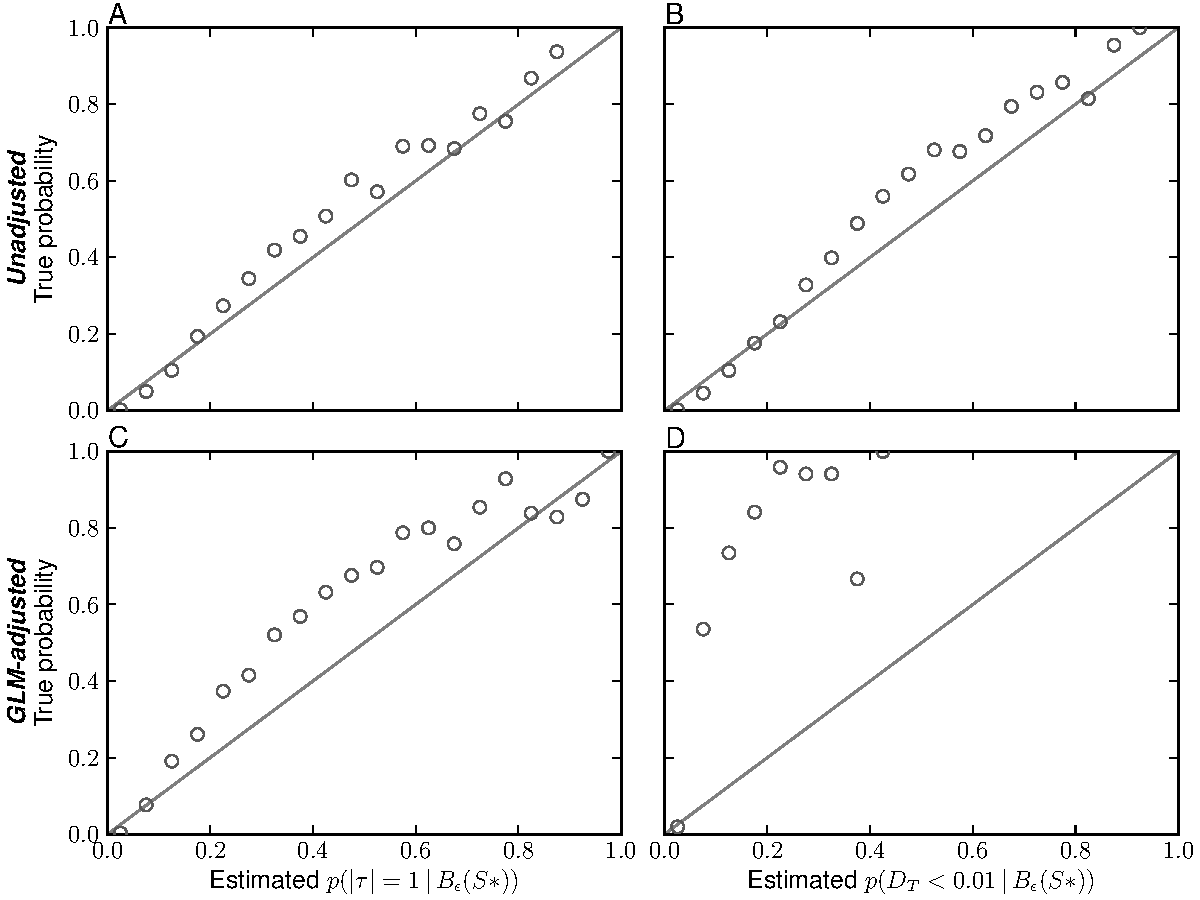
\includegraphics[width=1.0\textwidth]{../../validation/results/dpp/pymsbayes-results/plots/prior-dpp_prior-dpp_mc_behavior.pdf}
    \caption{
        Model-choice behavior \ldots
    }
    \label{fig_dpp_dpp_val_mc}
\end{figure}

\clearpage


%%%%%%%%%%%%%%%%%%%%%%%%%%%%%%%%%%%%%%%%%%%%%%%%%%%%%%%%%%%%%%%%%%
%% SUPPORTING INFO %%%%%%%%%%%%%%%%%%%%%%%%%%%%%%%%%%%%%%%%%%%%%%%
\setcounter{figure}{0}
\setcounter{table}{0}
\setcounter{page}{1}

\singlespacing

\renewcommand{\refname}{\noindent\MakeUppercase{\LARGE\sffamily\upshape Supporting Information}}

% PUT MAIN TEXT CITATION HERE
% \begin{thebibliography}{1}
% \providecommand{\natexlab}[1]{#1}
% \providecommand{\url}[1]{\texttt{#1}}
% \providecommand{\urlprefix}{URL }

% \bibitem

% \end{thebibliography}


%% SUPPL TABLES %%%%%%%%%%%%%%%%%%%%%%%%%%%%
%\setcounter{table}{0}


\end{document}

